\section{System Design}
\label{sec:design}
\label{sec:theory}
\label{sec:method}
% =====================================================================
% Merged from the prior \S4 Theoretical Framework and \S5 Methodology
% per the polish-pass M3(b) merge decision. Flattened to normal
% subsections per pre-submission review (avoids the prior "4.0.1"
% subsubsection numbering anomaly). All original cross-reference
% labels (sec:theory, sec:method, sec:t3-witnesses,
% sec:dt-calibration, sec:method-grammar) are preserved.
% =====================================================================

The canonical PG-DSL pipeline comprises four components that run as
a single pre-context-injection pass: (i) the \emph{lifter}
$L_{\text{verify}}$, (ii) the \emph{per-tool DT verifier}, (iii) the
\emph{composition-aware DT verifier} (which produces a blocked-pair
set later enforced by a runtime pair guard), and (iv) the
\emph{formal matcher}. Only tools whose claims survive both the
per-tool and composition verifications are exposed to the agent. The
remaining subsections describe each component and the three
conditional properties of the pipeline under bounded DT fidelity and
restricted grammar coverage --- T2 with the lifter (\S\ref{sec:design-lifter}),
T1${}_v$ with the per-tool DT verifier (\S\ref{sec:design-dt}), and
T3 with the composed defence (\S\ref{sec:design-t3}).

\subsection{Class $\mathcal{C}$ of CPS-Grounded Tool Descriptions}
\label{sec:method-grammar}

A description $D \in \mathcal{C}$ is a finite sequence of statements
drawn from the grammar
\[
\begin{aligned}
\text{statement} ::= {}&
  \text{actuator}(\textit{name}) := \textit{value} \\
&\mid\ \text{sensor}(\textit{name})\ \text{reads}\ \textit{value} \\
&\mid\ \Delta\text{state}(\textit{var})\ \{\textit{property}^{+}\}
\end{aligned}
\]
where $\textit{name}$ ranges over the SWaT P1+P2 vocabulary
(MV101, MV201, P101--P206, LIT101, FIT101, and AIT201--AIT203),
$\textit{value}$ over discrete actuator states or numeric sensor
readings, and $\textit{property}$ over monotone~$[\pm]$,
bounded~$[a, b]$, and sign~$[\pm 0]$. The grammar is locked for the
paper; the full Lark grammar is in Appendix~\ref{app:grammar}.

\subsection{Lifter $L_{\text{verify}}$ and T2 Lifting Soundness}
\label{sec:design-lifter}

\paragraph{Lifter.}
$L_{\text{verify}}$ is a locked LLM (\texttt{qwen3:14b} via Ollama at
\texttt{temperature}~$=0.0$, \texttt{seed}~$=42$, \texttt{think}~$=
\text{False}$ to disable thinking-mode token expenditure). The
\texttt{seed} is fixed for environment reproducibility; with $T=0$
and \texttt{think=False} the lifter is deterministic on a fixed
prompt and the seed value has no effect on the output token
distribution. The lifter prompt (``v1''/restrained) instructs the
model to lift \emph{only} explicit content from the description under
five restraint rules R1--R5 (Appendix~\ref{app:prompt}):
explicit-content-only, no-inferred-$\Delta$state, per-clause-lifting,
single-actuator-per-tool, and parametric-tool-minimal. R3--R5 were
added in the revision pass to close failure modes (co-actuator
inference, multi-pump enumeration) surfaced by the extended
out-of-family paraphrase corpus; the artifact ships both v1 variants
for ablation.

We define
\[
\varepsilon_L := \sup_{D \in \mathcal{C}} d\!\left(L_{\text{verify}}(D),
                                                 \varphi^{*}(D)\right),
\]
where $\varphi^{*}(D)$ is the ground-truth claim and $d(\cdot, \cdot)$
is a semantic distance over claims realised in sensor space as the
per-sample bias the lifter induces on the predicted trajectory.

\paragraph{T2 --- Lifting soundness decomposition.}
\begin{theorem}[T2, Lifting Soundness on Class $\mathcal{C}$]
\label{thm:t2}
For tool descriptions $D$ drawn i.i.d.\ from a distribution supported
on $\mathcal{C}$, the verifier LLM $L_{\text{verify}}$ produces a
sound formal claim with probability at least
$1 - \delta_{\text{lift}}$, where
\[
\delta_{\text{lift}}
\;\leq\;
\delta_{\text{cov}}(\mathcal{C}, L_{\text{verify}})
+ \delta_{\text{gram}}(\mathcal{C}),
\]
$\delta_{\text{cov}}$ is the LLM's error rate on $\mathcal{C}$ and
$\delta_{\text{gram}}$ is the rate at which honest descriptions fail
to admit any in-grammar lifting.
\end{theorem}

T2 is parametric in $\delta_{\text{lift}}$: the bound is a structural
decomposition rather than a numerical claim. Empirically, on
\texttt{qwen3:14b} with prompt v1 against a $227$-paraphrase benign
corpus (FORMAL/CASUAL/TERSE styles, generated by an out-of-family
paraphraser \texttt{mistral:7b}), we observe $\delta_{\text{lift}} =
0.44\%$ point estimate (Wilson 95\%~CI~$[0.08\%, 2.45\%]$); a single
CASUAL out-of-grammar rejection out of $227$ entries is the only
rejection. This is well within Req2LTL's prior estimate of
$\sim 11.6\%$ and tighter than the prior $42$-paraphrase corpus.

\subsection{Per-Tool DT Verifier and T1${}_v$ Detection Threshold}
\label{sec:design-dt}

\paragraph{Per-tool DT verifier.}
For each candidate tool, the DT verifier instantiates a fresh
\texttt{SwatP1P2Plant} digital twin~\cite{minicps} with the canonical
$14$-tool surface, sets one of three representative initial states
$\{\text{LOW}, \text{MID}, \text{HIGH}\}$ that sweep the operating
envelope, executes the candidate tool's implementation, and records
the trajectory $\psi$ over a $120$~s admission window. The matcher
checks $\varphi \models \psi$ per state-variable; a mismatch on any
of the three initial states rejects the tool from admission.

\paragraph{Notation.}
Let $\Sigma \subseteq \mathbb{R}^n$ denote the physical state space
relevant to admission verification, with state coordinates indexed by
$k \in \{1, \dots, n\}$. For the canonical SWaT P1+P2 substrate, the
level coordinates of interest at admission time are $(L_{T101},
L_{T201})$ ($n=2$). The admission target $T$ is either a single tool
description $D_i$ or an ordered pair $(D_i, D_j)$. The lifter
produces, for each coordinate $k$, an admissible region
$A_\varphi(k) \subseteq \mathbb{R}$ (or $\top$ if $\varphi_v$ does not
name coordinate $k$). The composition-aware verifier additionally
supplies an effective operating safe band $A_{\text{eff}}(k)$ from
runtime safety knowledge. The per-coordinate trajectory discrepancy
of the actual trajectory $\psi_v^{*}: [0, T_{\text{horizon}}] \to
\Sigma$ from the admissible region is
\[
\delta_v[k] := \sup_{t \in [0, T_{\text{horizon}}]}
   d_k\!\bigl(\psi_v^{*}(t)[k],\; A_{\text{eff}}(k)\bigr),
\]
with $d_k(x, [a,b]) = \max(0, x-b, a-x)$ and $d_k(x, \top) = 0$. The
vectorized magnitude is $\|\delta_v\|_\infty = \max_k \delta_v[k]$.

\paragraph{T1${}_v$ --- Vectorized detection threshold.}
\begin{theorem}[T1${}_v$, Vectorized Detection Threshold]
\label{thm:t1v}
Let $L_{\text{verify}}$ have vectorized semantic error
$\varepsilon_{L,v}$ on class $\mathcal{C}$ and let $\mathit{DT}$ have
vectorized per-sample fidelity error $\varepsilon_{DT,v}$, with
bounded errors per coordinate. For any admission target $T$ with
lifted vectorized claim $\varphi_v$ and actual trajectory $\psi_v^{*}$
whose discrepancy $\delta_v$ satisfies $\|\delta_v\|_\infty \geq \tau$,
the matcher's detection probability satisfies
\[
\Pr(\text{detect} \mid \|\delta_v\|_\infty \geq \tau)
   \;\geq\;
1 - F_v(\tau,\,\varepsilon_{L,v},\,\varepsilon_{DT,v}),
\]
where $F_v$ is monotone non-increasing in $\tau$. Under deterministic
bounded error,
\[
F_v(\tau,\,\varepsilon_{L,v},\,\varepsilon_{DT,v}) =
\begin{cases}
1 & \tau < \delta^{*}_{v} \\
0 & \tau \geq \delta^{*}_{v}
\end{cases},
\quad
\delta^{*}_{v} = 2\,\|\varepsilon_{L,v} + \varepsilon_{DT,v}\|_\infty;
\]
detection is guaranteed when $\|\delta_v\|_\infty > \delta^{*}_v$.
\end{theorem}

The proof (per-coordinate triangle inequality combined via max-norm)
is in Appendix~\ref{app:t1v-proof}.

\paragraph{Specialization to scalar T1.}
At $n=1$, $\|\delta_v\|_\infty = \delta$, $\delta^{*}_v =
2(\varepsilon_L + \varepsilon_{DT})$, and $F_v$ reduces to the
deterministic step of the scalar bounded-error analysis. T1${}_v$
strictly generalizes T1.

\paragraph{Concrete instantiation on the two-tank tractable model.}
Anchoring $\varepsilon_{L,v} = (0.116, 0.116)$ \%-full per coordinate
(Req2LTL accuracy gap~\cite{req2ltl}) and $\varepsilon_{DT,v} =
(0.10, 0.10)$ \%-full (per-sample matcher tolerance, calibration
details below) gives $\delta^{*}_v = 0.432$ \%-full.
Figure~\ref{fig:detection_v} shows the empirical detection rate from
a 1000-trial sweep on a two-tank coupled model matching the
theoretical 1 - $F_v$ step exactly; the $Z_3$ witness sits at
$\|\delta_v\|_\infty = 5.0$ \%-full ($11.6\times$ above the
bounded-error threshold, empirical detection $1.000$).

\begin{figure}[t]
\centering
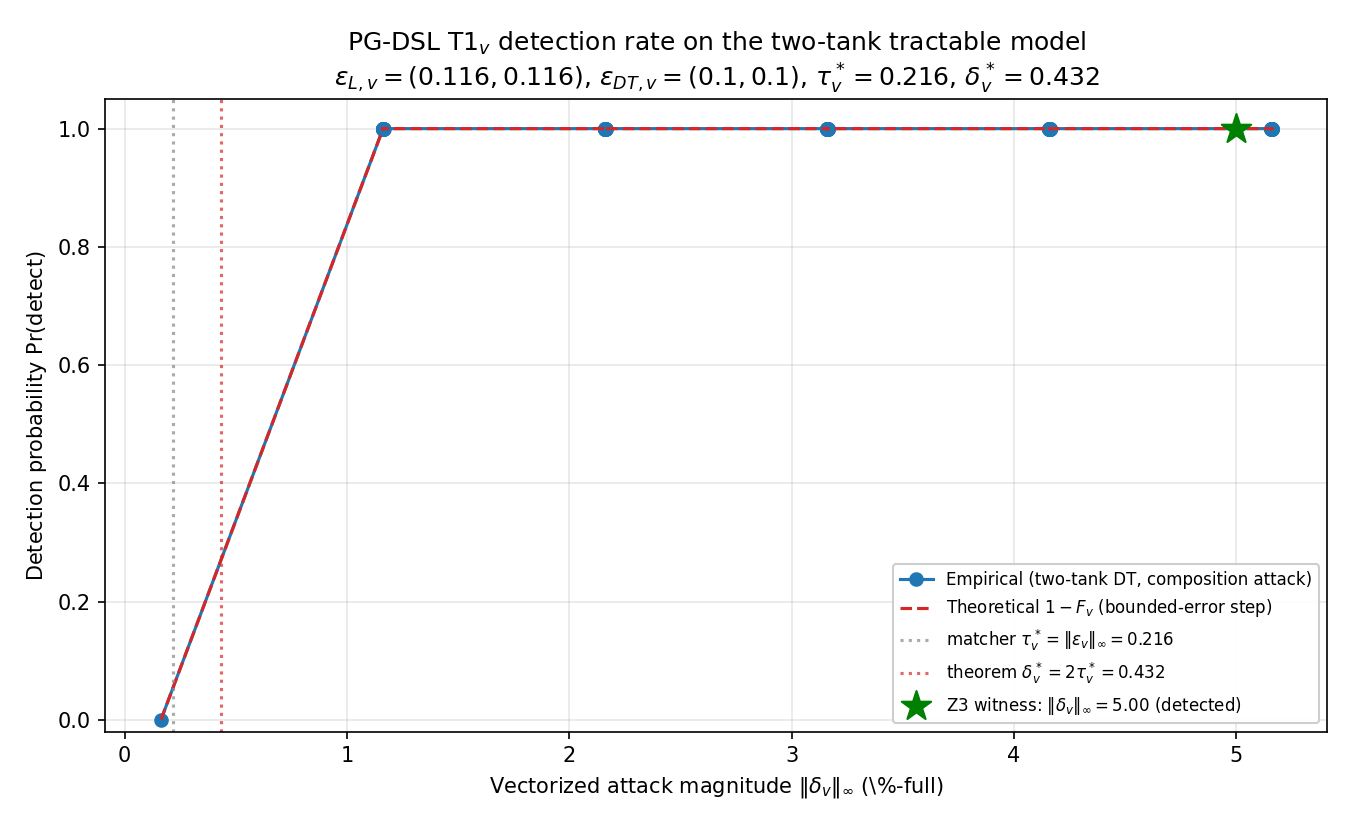
\includegraphics[width=0.95\columnwidth]{figures/detection_rate_plot_v.png}
\caption{Empirical detection rate (blue, two-tank tractable model;
1000 trials per bin) vs.\ theoretical $1 - F_v$ (dashed red step) at
$\delta^{*}_v = 0.432$ \%-full. $Z_3$ witness (green star at
$\|\delta_v\|_\infty = 5.0$, detection $1.000$) sits in the detected
region. $\varepsilon_{L,v} = (0.116, 0.116)$, $\varepsilon_{DT,v} =
(0.10, 0.10)$.}
\label{fig:detection_v}
\end{figure}

\paragraph{$\varepsilon_{DT}$ calibration and sensitivity.}
\label{sec:dt-calibration}
We distinguish the \emph{per-sample matcher tolerance}
$\varepsilon_{DT}$ used in the T1${}_v$ admission matcher from the
\emph{full-transient residual envelope}. The paper-canonical
$\varepsilon_{DT} = 0.10$ \%-full is the median of the per-sample
$|\Delta L_{T101}|$ distribution on $10$ benign-baseline trajectories
(rounded up to the nearest $0.05$ \%-full LIT-sensor granularity);
this is the appropriate calibration for the matcher because the
admission replay compares \emph{steady post-action} state summaries
rather than worst-case transients. The full-transient envelope is
larger: the $99.5$th percentile of the same per-sample residual
distribution reaches $0.40$ \%-full at full transient; using this
conservative bound as $\varepsilon_{DT}$ would raise $\delta^{*}_v$
from $0.432$ to $1.032$ \%-full. Both thresholds are reported below.
The T1${}_v$ deterministic threshold $\delta^{*}_v =
2(\varepsilon_L + \varepsilon_{DT})$ is monotone in
$\varepsilon_{DT}$: $\varepsilon_{DT} \in \{0.05, 0.10, 0.20, 0.40\}$
gives $\delta^{*}_v \in \{0.332, 0.432, 0.632, 1.032\}$ \%-full. The
$Z_3$ witness's $\|\delta_v\|_\infty = 5.0$ sits at $\{15.06\times,
11.57\times, 7.91\times, 4.85\times\}$ above the threshold
respectively; detection is robust across the calibration window,
including the conservative $99.5$th-percentile-transient bound.

\subsection{Composition-Aware DT Verifier and Runtime Pair Enforcement}

The composition-aware verifier replays each ordered pair
$(D_i, D_j)$ of admitted-actuator tools from each of $\{\text{LOW},
\text{MID}, \text{HIGH}\}$ in a fresh DT for $30$~s, then flags pairs
whose composed trajectory exits the runtime safety band
$[25, 95]$ \%-full for $L_{T101}$ or $[20, 95]$ for $L_{T201}$. The
verdict outputs a \emph{blocked-pair set}; tools remain individually
admitted but the runtime guard rejects calls to an ordered pair in
the blocked set. Reads and the parametric \texttt{set\_dosing\_rate}
are excluded from composition replay (no side effects / parametric
tool covered by the per-tool layer). This component performs
admission-time pair analysis but the enforcement happens at
\emph{runtime}: PG-DSL is admission-time \emph{filtering} for
single-tool descriptions and admission-time \emph{pair analysis with
runtime pair enforcement} for compositions.

The composition pass tests $|\mathit{admitted}_{\text{actuator}}|^2
\cdot 3$ ordered (pair, init-state) tuples in worst case; on the
canonical $14$-tool surface this is $168$ replays of negligible cost
($\sim 0.2$~s) compared to the per-tool admission cost (lifter
inference dominates). For surfaces beyond a few hundred tools, a
heuristic pre-filter --- e.g., a monotone sign-classifier on
actuator semantics that rejects pairs with no actuator-state
intersection --- would prune the $O(k^2 \cdot |\mathcal{I}|)$ replay
budget without loss of coverage; we leave this engineering
optimization to future work.

\subsection{Formal Matcher}

The matcher walks each clause in $\varphi$ and checks satisfaction in
$\psi$ within per-state-variable tolerance:
\begin{itemize}
\item $\text{actuator}(N) := v$: pass iff
      $\psi.\text{actuator\_post}[N] = v$ (binary, exact).
\item $\text{sensor}(N)\ \text{reads}\ V$: pass iff the tool's
      return value equals the named sensor's oracle read within
      $\varepsilon_{DT}$.
\item $\Delta\text{state}(\textit{var})\,\{\textit{prop}\}$: pass iff
      the per-state-variable trajectory summary respects the claimed
      \texttt{sign}/\texttt{monotone}/\texttt{bounded} property within
      tolerance.
\end{itemize}
The matcher's tolerances follow T1${}_v$: $\varepsilon_{DT} = 1.0$
\%-full per sample for level coordinates; $\varepsilon_{DT} = 0.05$
on AIT201 conductivity (one-tenth of the band width).

\subsection{T3 --- Strict-Composition Witness with Runtime CPS-IDS}
\label{sec:design-t3}
\label{sec:t3-witnesses}

\begin{theorem}[T3, Strict-Composition Witness]
\label{thm:t3}
Let $A_{\text{static}}$ be the set of attacks canonical PG-DSL
detects at admission, and $A_{\text{runtime}}$ the set detected by a
runtime CPS-IDS $\mathcal{I}$ (e.g.\ INVARLLM~\cite{invarllm}). On
the canonical 8-attack set defined in this paper, $A_{\text{static}}
\setminus A_{\text{runtime}} \neq \emptyset$ and $A_{\text{runtime}}
\setminus A_{\text{static}} \neq \emptyset$. Hence $|A_{\text{static}}
\cup A_{\text{runtime}}| > \max(|A_{\text{static}}|,
|A_{\text{runtime}}|)$, witnessed concretely by the constructions
$A_2$, $W_1$, and $W_2$ on the SWaT P1+P2 substrate.
\end{theorem}

T3 is a witnessed strict-superset property on the canonical attack
set, not a general security theorem; the witnesses establish that the
admission-time and runtime defences cover complementary visibility
surfaces on this substrate.

\paragraph{$W_{T3,A_2}$ --- $A_{\text{static}} \setminus A_{\text{runtime}}$.}
\textit{Setup.} \texttt{set\_dosing\_rate} description claims
$0.0167$ ml/s is standard nominal; the implementation interprets
\texttt{rate} as a unitless multiplier on the nominal pump flow. The
agent supplies $0.0167$ per the description; the plant runs at
$60\times$ underdose. Within the $120$~s admission window, AIT201
fails to rise above $0.4$.
\textit{INVARLLM behaviour.} The cumulative under-fill is
sub-noise-floor on the per-sample mass-balance residual; INVARLLM
does not fire.
\textit{Canonical PG-DSL behaviour.} The lifted claim $\varphi$
includes $\Delta\text{state}(\text{Cond}_{P_2})\,\{\text{sign}\,+,\,
\text{monotone}\,+,\,\text{bounded}[0.40, 1.50]\}$; the DT replay
against the attacker-supplied rate ends with AIT201 below the bounded
band and the matcher fires deterministically.

\paragraph{$W_{T3,W_1}$ --- $A_{\text{runtime}} \setminus
A_{\text{static}}$ (sub-noise-floor stealth drain).}
\textit{Setup.} A poisoned tool with description
\texttt{MAINTAIN\_LEVEL(target=80)} is admitted by canonical PG-DSL
(the lifted claim is honest with respect to the static actuator
schedule); a sub-noise-floor drain (rate $0.025$ \%-full/s, below the
$0.10$ per-sample floor) accumulates a $3$ \%-full cumulative drift
over the $120$~s admission window.
\textit{INVARLLM behaviour.} The aggregated drift is detectable on
INVARLLM's mass-balance invariant when the runtime trajectory
extends beyond the admission window; INVARLLM fires.
\textit{Canonical PG-DSL behaviour.} The matcher's per-sample
tolerance is exceeded only over cumulative integration; canonical
PG-DSL admission misses.

\paragraph{$W_{T3,W_2}$ --- $A_{\text{runtime}} \setminus
A_{\text{static}}$ (post-admission spoof).}
\textit{Setup.} \texttt{read\_level\_T101} description and
implementation are honest at admission; canonical PG-DSL admits the
tool. After admission, an attacker spoofs the LIT101 reading to a
constant $80\%$ at the network layer while pumps drive the tank to
overflow.
\textit{Canonical PG-DSL behaviour.} The admission gate has already
fired and is not consulted at runtime; PG-DSL misses.
\textit{INVARLLM behaviour.} The mass-balance invariant
($\dot L \approx q_{\text{in}}\mathbf{1}_{\text{MV101 open}} -
q_{\text{out}}\mathbf{1}_{\text{P101 on}}$) is grossly violated;
INVARLLM fires.

\paragraph{Witness partition under canonical PG-DSL.}
The composition-aware DT verifier additionally moves $Z_3$ (transient
overshoot via admitted-tool composition) from $A_{\text{runtime}}$
into $A_{\text{static}} \cap A_{\text{runtime}}$: each constituent
tool admits per-tool, but the ordered pair
$(\text{open\_valve\_MV101}, \text{start\_pump\_P101})$ from the
\texttt{HIGH} initial state ($L_{T101} = 90$ \%-full) replays to a
band-exit at $t = 11$~s and overflow at $t = 19$~s, so the canonical
matcher rejects the pair; the runtime pair guard then prevents the
agent from executing the pair. T1${}_v$'s detected region predicts
this catch: $\|\delta_v\|_\infty = 5.0 \gg \delta^{*}_v = 0.432$.

The empirical T3 partition under canonical PG-DSL $\oplus$ INVARLLM is
\begin{align*}
A_{\text{static}} \setminus A_{\text{runtime}} &= \{A_2\}, \\
A_{\text{runtime}} \setminus A_{\text{static}} &= \{W_1, W_2\}, \\
A_{\text{static}} \cap A_{\text{runtime}} &= \{A_1, A_3, Z_1, Z_2, Z_3\}, \\
A_{\text{static}} \cup A_{\text{runtime}} &= \text{all 8 attacks}.
\end{align*}
Both strict-difference directions are non-empty and the composed
defence covers the canonical attack set (canonical pipeline T3
partition results released with the artifact). The witnessed
strict-superset property holds on the canonical 8-attack set under
the witness constructions above; T3 is a witnessed composition
result on this substrate, not a general security statement.

\subsection{Implementation}

The implementation comprises Python modules organised by concern:
the \emph{plant module} (plant simulator, MCP server, attack
mountings), the \emph{per-tool admission module} (lifter, DT
verifier, matcher, single-tool admission orchestrator), and the
\emph{canonical pipeline module} (canonical PG-DSL = per-tool
$\oplus$ composition orchestrator). The MCP server speaks real
JSON-RPC 2.0 over stdio per the official MCP
specification~\cite{mcp_spec}, consumable by the official Python MCP
SDK and equivalent third-party agent harnesses. Both deterministic
stub and \texttt{qwen3:14b} configurations are reproduced by the
artifact.

% =====================================================================
